

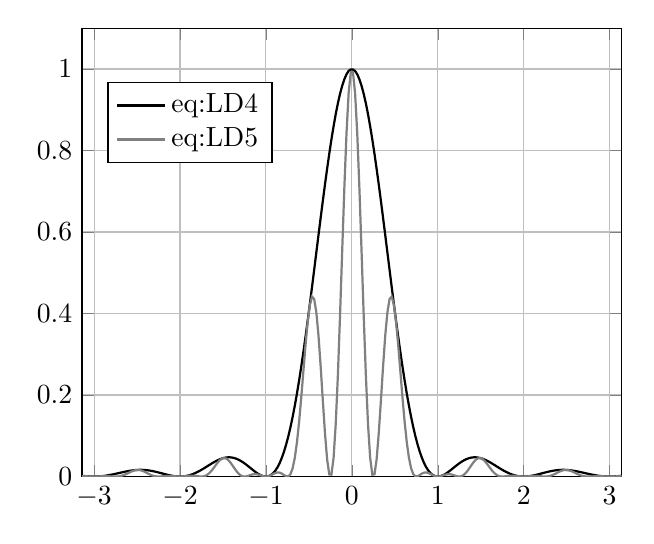
\begin{tikzpicture}
  \begin{axis}[
    samples=400,
    xlabel={},
    ylabel={},
    ymin=0, ymax=1.1,
    xmin=-3.14,xmax=3.14,
    legend style={at={(0.2,0.7)}, anchor=south},
    grid=major,
  ]
    % sinc^2(x)
    \addplot[
      thick
    ] { (sin(deg(pi*x))/(pi*x))^2 };
    \addlegendentry{\cref{eq:LD4}}
    
    % sinc^2(x) * cos^2(x)
    \addplot[
      thick,
      gray
    ] { (sin(deg(pi*x))/(pi*x))^2 * (cos(deg(2*pi*x)))^2 };
    \addlegendentry{\cref{eq:LD5}}
  \end{axis}
\end{tikzpicture}

